% !TEX encoding = UTF-8
% !TEX TS-program = pdflatex
% !TEX root = ../tesi.tex

%**************************************************************
\chapter{Introduzione}
\label{cap:introduzione}
%**************************************************************

Al giorno d'oggi la tecnologia sta ricoprendo un ruolo importante nei \textit{task} di tutti i giorni. In particolare, è indispensabile che un'azienda venditrice di un qualsiasi tipo di prodotti abbia una propria \glossaryItem{piattaforma} \textit{online} per la gestione degli ordini. Questo perché le persone sono sempre più abituate ad effettuare ordini \textit{online}. Infatti, acquistare \textit{online} risulta vantaggioso per molteplici motivi, quali il risparmio di tempo e denaro ma soprattutto la comodità di non doversi muovere da casa per acquistare un prodotto. Per molte aziende non cogliere questo cambiamento potrebbe essere fallimentare, infatti, in futuro, la maggior parte degli acquisti avverrà principalmente \textit{online} per qualsiasi tipologia di prodotto. 

\textit{MoviORDER} nasce per rispondere a questa necessità, proponendosi come piattaforma universale per la registrazione e l'invio di ordini \textit{online}. Una qualsiasi azienda interessata a vendere i propri prodotti \textit{online} può contattare \visione{} per ricevere \textit{moviORDER} e, dopo un breve periodo di configurazione, l'applicazione sarà pronta a ricevere ordini dagli utenti registrati. 
\textit{MoviORDER} risulta vantaggiosa per i seguenti motivi:
\begin{itemize}
	\item per i clienti:
	\begin{itemize}
		\item possibilità di trovare i prodotti \textit{online} e non solamente nel negozio fisico;
		\item possibilità di risparmiare tempo e denaro dovuti al raggiungimento del negozio fisico;
		\item possibilità di controllare in tempo reale la disponibilità dei prodotti.
	\end{itemize}
	\item per le aziende:
	\begin{itemize}
		\item riduce il rischio di fallimento dovuto al cambiamento delle convenzioni degli utenti;
		\item aumenta il numero di clienti per l'azienda, permettendo a coloro che non riescono a raggiungere il negozio fisico di poter comunque effettuare ordini grazie alla piattaforma \textit{online}.
	\end{itemize}
\end{itemize}

%**************************************************************
\section{L'azienda}

\visione{} è un'azienda che da 30 anni si occupa di informatica e più precisamente di quella parte dell'informatica dedicata alle applicazioni gestionali. Inizialmente l'attività di \visione{} era rivolta ad aziende, enti pubblici, studi professionali e centri di elaborazione dati, gestendo totalmente problematiche informatiche, progettazione di sistemi, \textit{hardware}, reti, sistemi operativi e \textit{software} applicativo. Oggi \visione{} punta sulla specializzazione, dedicandosi in modo particolare allo sviluppo del \textit{software} applicativo e dei relativi servizi di implementazione dello stesso nell'azienda. \visione{} è un \textit{team} di persone esperte e motivate che opera direttamente su gran parte del Nord Est e indirettamente sull'intero territorio nazionale. \visione{} si rivolge a piccole e medie aziende italiane che intendono impostare sul sistema informatico non solo la semplice gestione amministrativa o di magazzino, ma la completa organizzazione aziendale per affrontare un futuro sempre più complesso e veloce, con il supporto di un sistema informatico che aiuti l'azienda a prendere decisioni sempre basate su dati precisi.

\begin{figure}[!h] 
    \centering 
    
\includegraphics[width=0.6\columnwidth]{visione/logoVisione} 
    \caption{Logo dell'azienda \visione{}}
\end{figure}

\subsection{\textit{Core business}}

\visione{} presenta principalmente due \textit{core business}: \textit{VisionENTERPRISE} e \textit{movidat}. \textit{VisionENTERPRISE} è un \glossaryItem{software gestionale} \glossaryItem{ERP} dedicato alle medie e piccole aziende industriali, commerciali e dei servizi, che gestiscono notevoli moli di dati e hanno la necessità di lavorare con grande velocità e stabilità. Il \textit{software} è in grado di collegarsi a tutte le informazioni dell'azienda cliente e di interfacciarsi con tutti i \textit{software} utilizzati al fine di gestire in modo ottimale l'intera organizzazione aziendale con la massima semplicità e velocità operativa. Il \textit{software} è in grado di rendere disponibile in tempo reale, alla direzione o al titolare dell'azienda, tutte le informazioni di cui hanno bisogno per prendere decisioni sulla base di dati concreti e oggettivi. Altra qualità di \textit{VisionENTERPRISE} è la sua completa copertura funzionale: dalla contabilità al magazzino, dall'area commerciale alla produzione, dal controllo di gestione all'\glossaryItem{E-business}.

\begin{figure}[!h] 
    \centering 
    
\includegraphics[width=0.8\columnwidth]{visione/visionEnterprise} 
    \caption{Banner del \textit{software} \textit{VisionENTERPRISE}}
\end{figure}

\textit{Movidat} è un marchio di \visione{} che progetta e sviluppa applicazioni per dispositivi \textit{mobile} rivolte alle piccole e medie imprese che vogliono rendere i loro processi più semplici, veloci ed efficienti. Lo slogan di \textit{movidat} è ``ovunque tu sia, il tuo \textit{business} a portata di mano!'', infatti le applicazioni \textit{movidat} sono rivolte ai dipendenti che lavorano in movimento, i quali devono essere in grado di agire tempestivamente in caso di problematiche inaspettate. Le soluzioni \textit{movidat} sono compatibili con la maggior parte dei \textit{software} gestionali disponibili sul mercato. Tra le soluzioni di miglior successo vi sono:
\begin{itemize}
	\item \textbf{\textit{moviCheck}}: applicazione rivolta alle aziende che vogliono offrire alle proprie figure direzionali uno strumento in grado di analizzare in mobilità i dati di \textit{business} più significativi;
	\item \textbf{\textit{moviSell}}: applicazione specificatamente rivolta ai professionisti della vendita, ideata come supporto per la gestione dei rapporti con i clienti.
\end{itemize}

\begin{figure}[!h] 
    \centering 
    
\includegraphics[width=0.6\columnwidth]{visione/movidat} 
    \caption{Logo del marchio \textit{movidat}}
\end{figure}

\textit{MoviORDER} rientra tra le applicazioni del marchio \textit{movidat}, soddisfacendo però i bisogni del cliente finale dell'azienda. Infatti, tramite \textit{moviORDER}, gli utenti possono acquistare dei prodotti della propria azienda direttamente \textit{online}, senza doversi recare al negozio fisico.

%**************************************************************
\section{Offerta di \textit{stage}}

Il 10 Aprile 2018 si è tenuta a Padova la 15-esima edizione di \textit{Stage-IT}, iniziativa che mira ad agevolare l'incontro tra aziende e studenti universitari che puntano ad entrare nel mondo del lavoro con specifico riferimento al settore \glossaryItem{ICT}, favorendo un'occasione di conoscenza reciproca tramite colloqui individuali. Le aziende partecipanti propongono spesso progetti innovativi con ottime opportunità di accrescimento delle competenze individuali. Proprio per questo motivo, lo stagista ha deciso di partecipare attivamente all'evento, concludendo positivamente sette colloqui. 

\begin{figure}[!h] 
    \centering 
    
\includegraphics[width=0.8\columnwidth]{loghi/stage} 
    \caption{Logo dell'evento \textit{Stage-IT}}
\end{figure}

Le aziende sono state selezionate dallo studente per ambito e tecnologie di sviluppo adottate nel progetto. In particolare, lo studente era in cerca di:
\begin{itemize}
	\item progetti di sviluppo in ambito \textit{mobile} (preferibilmente \textit{Android}): al giorno d'oggi i \textit{task} si stanno spostando sempre di più dalle postazioni \textit{desktop} ai dispositivi portatili;
	\item progetti di sviluppo di \glossaryItem{applicazioni web} (preferibilmente con utilizzo di \textit{framework} e \glossaryItem{librerie} \textit{Javascript} moderne): le \textit{skill} di programmazione in \textit{Javascript} sono richieste da gran parte delle aziende che si occupano della realizzazione di applicazioni \textit{web}.
\end{itemize}
Tra le varie offerte di \textit{stage}, \visione{} rientrava in entrambe le preferenze, infatti proponeva un progetto di sviluppo in ambito \textit{mobile} con l'utilizzo di un \textit{framework cross-platform}. Nonostante lo \textit{stage} non prevedesse lo sviluppo in \glossaryItem{codice nativo} \textit{Android}, permetteva comunque la realizzazione di un'applicazione \textit{mobile}. Inoltre, richiedendo il progetto l'utilizzo di un \textit{framework cross-platform}, era pressoché implicito l'utilizzo di \glossaryItem{tecnologie web}, tra le quali anche \textit{Javascript}. Per cui, il buon compromesso tra tecnologie conosciute e tecnologie ritenute interessanti ha favorito \visione{} tra le varie offerte analizzate.

\newpage

\section{Obiettivi e pianificazione}

Il progetto prevedeva la realizzazione di un'applicazione \textit{mobile}, principalmente \textit{Android} e \textit{iOS}, che consentisse ad un utente registrato, tramite la lettura di codici a barre o l'inserimento manuale di codici articolo, di inviare ordini di acquisto al proprio fornitore. L'azienda ha richiesto lo sviluppo delle seguenti funzionalità:
\begin{itemize}
	\item \textbf{\textit{login}}: permette ad un utente di essere riconosciuto come cliente dell'azienda. Le credenziali di accesso vengono distribuite dall'azienda insieme all'applicazione;
	\item \textbf{gestione del carrello}:
	\begin{itemize}
		\item \textbf{aggiunta di un nuovo articolo}: permette all'utente autenticato di aggiungere un nuovo articolo al carrello. L'aggiunta di un nuovo articolo prevede l'inserimento di un codice articolo, tramite scansione di un codice a barre o inserimento manuale e, successivamente, l'inserimento di una quantità da ordinare;
		\item \textbf{modifica di un articolo}: permette all'utente autenticato di modificare la quantità di un articolo in carrello;
		\item \textbf{selezione articoli}: permette all'utente autenticato di selezionare uno o più articoli in carrello;
		\item \textbf{deselezione articoli}: permette all'utente autenticato di deselezionare uno o più articoli in carrello;
		\item \textbf{rimozione articoli}: permette all'utente autenticato di rimuovere gli articoli selezionati dal carrello;
		\item \textbf{invio ordine}: permette all'utente autenticato di inviare un ordine composto dagli articoli selezionati in carrello.
	\end{itemize}
	\item \textbf{invio di \textit{e-mail} di conferma}: nel caso in cui un ordine venga inviato con successo, il sistema deve inviare all'azienda e all'utente autenticato una \textit{mail} di conferma contenente un riepilogo dell'ordine.
\end{itemize}

\hspace{-15pt}I prodotti attesi per il termine dello \textit{stage} erano:
\begin{itemize}
	\item \textbf{analisi dei requisiti} per l'applicazione da realizzare: partendo dalle specifiche e dalla microanalisi ricevuta, lo stagista doveva definire le funzionalità offerte dall'applicazione, i dettagli dei \textit{web services} di comunicazione tra \textit{database} e \glossaryItem{front end}, e l'interfaccia grafica dell'applicazione;
	\item \textbf{applicazione \textit{moviORDER}}: sviluppo dell'applicazione in ambiente \glossaryItem{multipiattaforma} in seguito alla scelta del \textit{framework} ritenuto più opportuno;
	\item \textbf{servizio \textit{web}}: sviluppo di un servizio \textit{web} che permettesse all'applicazione di accedere ed interagire con un \textit{database} su un \textit{server cloud} di \visione{};
	\item \textbf{manuali} utente e sviluppatore. 
\end{itemize}

Per adempiere a questi obblighi lo stagista ha pianificato delle attività che sono state concordate con il \textit{tutor} aziendale. Lo \textit{stage} prevedeva 320 ore di lavoro che sono state distribuite nel periodo tra l'inizio e la fine dello \textit{stage}, 2 Luglio 2018 e 7 Settembre 2018 rispettivamente. La pianificazione oraria delle attività all'inizio dello \textit{stage} è indicata nella seguente tabella.

{\renewcommand{\arraystretch}{2}
\begin{center}
\begin{longtable}{ | >{\arraybackslash}p{11cm} | >{\centering\arraybackslash}p{1cm} | }
        
\hline
\textbf{Attività} & \textbf{Ore} \\ \hline
\endhead
Formazione assistita sui \textit{software} gestionali di \visione{} e sulle applicazioni analoghe a \textit{moviORDER} & 40 \\ \hline
Formazione individuale sui \textit{framework cross-platform} e scelta del \textit{framework} ritenuto più opportuno & 40 \\ \hline
Ridefinizione delle specifiche comprendente delle soluzioni da realizzare e delle metodologie per implementarle & 40 \\ \hline
Realizzazione dei \textit{web services} per l'interazione con il \textit{database}: servizio di autenticazione, servizio di lettura dati, servizio di scrittura dati e servizio di invio \textit{e-mail} & 40 \\ \hline
Realizzazione della \textit{business logic} dell'applicazione & 40 \\ \hline
Realizzazione delle interfacce grafiche dell'applicazione: \textit{login}, gestione carrello, aggiunta/modifica articolo e invio ordine & 40 \\ \hline
Test di scambio dati tra \textit{VisionENTERPRISE} e \textit{moviORDER} & 40 \\ \hline
Documentazione del codice e stesura del manuale utente e sviluppatore & 40 \\
\hline
\caption{Pianificazione oraria del periodo di \textit{stage}}
\end{longtable}
\end{center}}

Viene di seguito riportato un \glossaryItem{diagramma di Gantt} che illustra come le attività di \textit{stage} sono state allocate nel tempo di calendario da parte dello stagista. Il diagramma mostra le dipendenze temporali tra le varie attività e il periodo di ferie che l'azienda ha concesso allo stagista, indicato in viola.

\begin{figure}[!h] 
    \centering 
    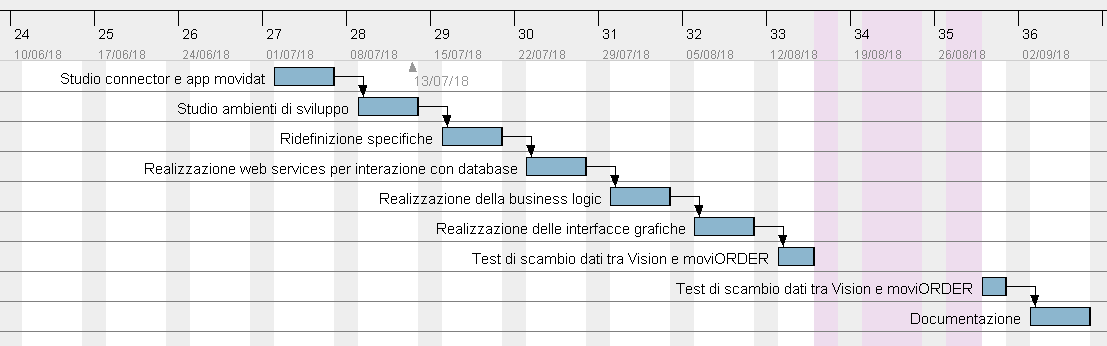
\includegraphics[width=\columnwidth]{diagrammi/pianificazione} 
    \caption{Diagramma di \textit{Gantt} della pianificazione delle attività di \textit{stage}}
\end{figure}

\newpage

\section{Rischi}

Parallelamente allo studio dei documenti forniti dal \textit{tutor} aziendale, è stata sviluppata un'analisi preventiva dei rischi che si sarebbero potuti verificare durante lo svolgimento delle attività di progetto. Al fine di attuare una corretta e quindi utile gestione dei rischi, essi sono stati identificati nel contesto di processo e di prodotto. In seguito all'identificazione dei rischi sono state analizzate le probabilità di occorrenza, imminenza e l'impatto di ciascun rischio, pianificando come evitarne o mitigarne gli effetti. Durante lo svolgimento del progetto è stato costantemente eseguito un controllo per rilevare eventuali indicatori di rischio e ogni nuovo rischio rilevato è stato aggiunto alla seguente tabella, insieme alle azioni atte a mitigarne gli effetti.

\begin{small}
    \begin{center}
        \renewcommand{\arraystretch}{2}
        \begin{longtable}{| >{\centering\arraybackslash}p{1.5cm} | >{\arraybackslash}p{4cm} | >{\centering\arraybackslash} p{2cm} | >{\arraybackslash} p{3.75cm}|}
        	\hline
            \textbf{Rischio} & \textbf{Descrizione} & \textbf{Grado} & \textbf{Mitigazione} \\
            \hline
            \endhead
            
            Tecnologie non conosciute
            &
            Il tempo richiesto per l'apprendimento delle nuove tecnologie da parte dello stagista
            potrebbe causare ritardi nello sviluppo
            &
            Occorrenza: \textbf{Media} Pericolosità: \textbf{Media}
            &
            Effettuare una buona analisi iniziale delle tecnologie richieste ed usufruire del tempo di formazione per prendere dimestichezza con le tecnologie non conosciute
         	\\
            \hline
            
            Modifica dei requisiti
            &
            Nonostante i requisiti esposti inizialmente siano chiari, vi è la possibilità
            che questi vengano modificati dal \textit{tutor} aziendale
            &
            Occorrenza: \textbf{Bassa} Pericolosità: \textbf{Alta}
            & 
            Negoziare la modifica ai requisiti nel caso in cui siano richiesti cambiamenti eccessivi da parte del \textit{tutor} aziendale
            \\
            \hline
            
            Stima dei tempi
            &
            Può accadere che lo stagista abbia pianificato erroneamente alcune attività e che durante lo sviluppo si sforino i tempi concordati
            &
            Occorrenza: \textbf{Media} Pericolosità: \textbf{Alta}
            & 
            Agire tempestivamente sulla pianificazione, ove possibile, nei casi più gravi. Pianificare in maniera intelligente inserendo dei \glossaryItem{periodi di slack} tra le attività ritenute più critiche
            \\
            \hline
            
            Difficoltà nelle interazioni
            &
            Durante lo \textit{stage} le interazioni avvengono spesso tramite scambio di \textit{e-mail} tra lo stagista e il \textit{tutor} aziendale. Può succedere che alcune risposte arrivino in tempi prolungati, causando tempi morti nello sviluppo dell'applicazione
            &
            Occorrenza: \textbf{Bassa} Pericolosità: \textbf{Media}
            & 
            Se il problema dovesse diventare ingestibile, proporre al tutor aziendale l'utilizzo di uno strumento di comunicazione alternativo, altrimenti presentarsi fisicamente in ufficio per discutere delle problematiche di maggiore entità
            \\
            \hline
            \caption{Analisi dei rischi}
        \end{longtable}
    \end{center}
\end{small}


%**************************************************************
\section{Organizzazione del testo}

\begin{description}
    \item[{\hyperref[cap:processi-metodologie]{Il secondo capitolo}}] descrive il modello di \glossaryItem{ciclo di vita} adottato durante lo sviluppo del progetto.
    
    \item[{\hyperref[background]{Il terzo capitolo}}] descrive le tecnologie utilizzate durante lo sviluppo del progetto.
    
    \item[{\hyperref[cap:analisi-requisiti]{Il quarto capitolo}}] descrive i \glossaryItem{casi d'uso} e i corrispondenti requisiti rilevati durante la fase di analisi dei requisiti del progetto.
    
    \item[{\hyperref[cap:progettazione-codifica]{Il quinto capitolo}}] descrive l'\glossaryItem{architettura} dell'applicazione, comprensiva di contestualizzazione dei \glossaryItem{design pattern} adottati.
    
    \item[{\hyperref[codifica]{Il sesto capitolo}}] descrive i dettagli implementativi del progetto.
    
    \item[{\hyperref[cap:verifica-validazione]{Il settimo capitolo}}] descrive i processi di verifica e validazione attuati nel progetto.
    
    \item[{\hyperref[cap:conclusioni]{L'ottavo capitolo}}] descrive le conclusioni tratte dallo studente in merito al progetto realizzato.
\end{description}

Riguardo la stesura del testo, relativamente al documento, sono state adottate le seguenti convenzioni tipografiche:
\begin{itemize}
	\item gli acronimi, le abbreviazioni e i termini ambigui o di uso non comune menzionati vengono definiti nel glossario, situato alla fine del presente documento in appendice §\ref{gloss};
	\item per la prima occorrenza dei termini riportati nel glossario viene utilizzata la seguente nomenclatura: \glossaryItem{termine};
	\item i termini in lingua straniera, o facenti parti del gergo tecnico, sono evidenziati con il carattere \emph{corsivo}.
\end{itemize}